\begin{frame}{Anchor words}
\begin{definition}
An \textbf{anchor word} is a word that appears with \emph{high} probability in one topic but with \emph{low} probability in all other topics.
\end{definition}
\end{frame}

\begin{frame}{From Co-occurrence to Topics}
\begin{itemize}
\item Normally, we want to find \(p(\text{word} \g \text{topic}) \)~\citep{blei-2003}.
\item Instead, what if we can easily find \(p(\text{word} \g \text{topic})\) through using anchor words and conditional word co-occurrence \(p(\text{word 2} \g \text{word 1})\)?
\end{itemize}
\end{frame}


\begin{frame}{From Co-occurrence to Topics}
\begin{equation*}
\bar{Q}_{i,j} = p(w_2 = j \g w_1 = i)
\end{equation*}
\begin{figure}
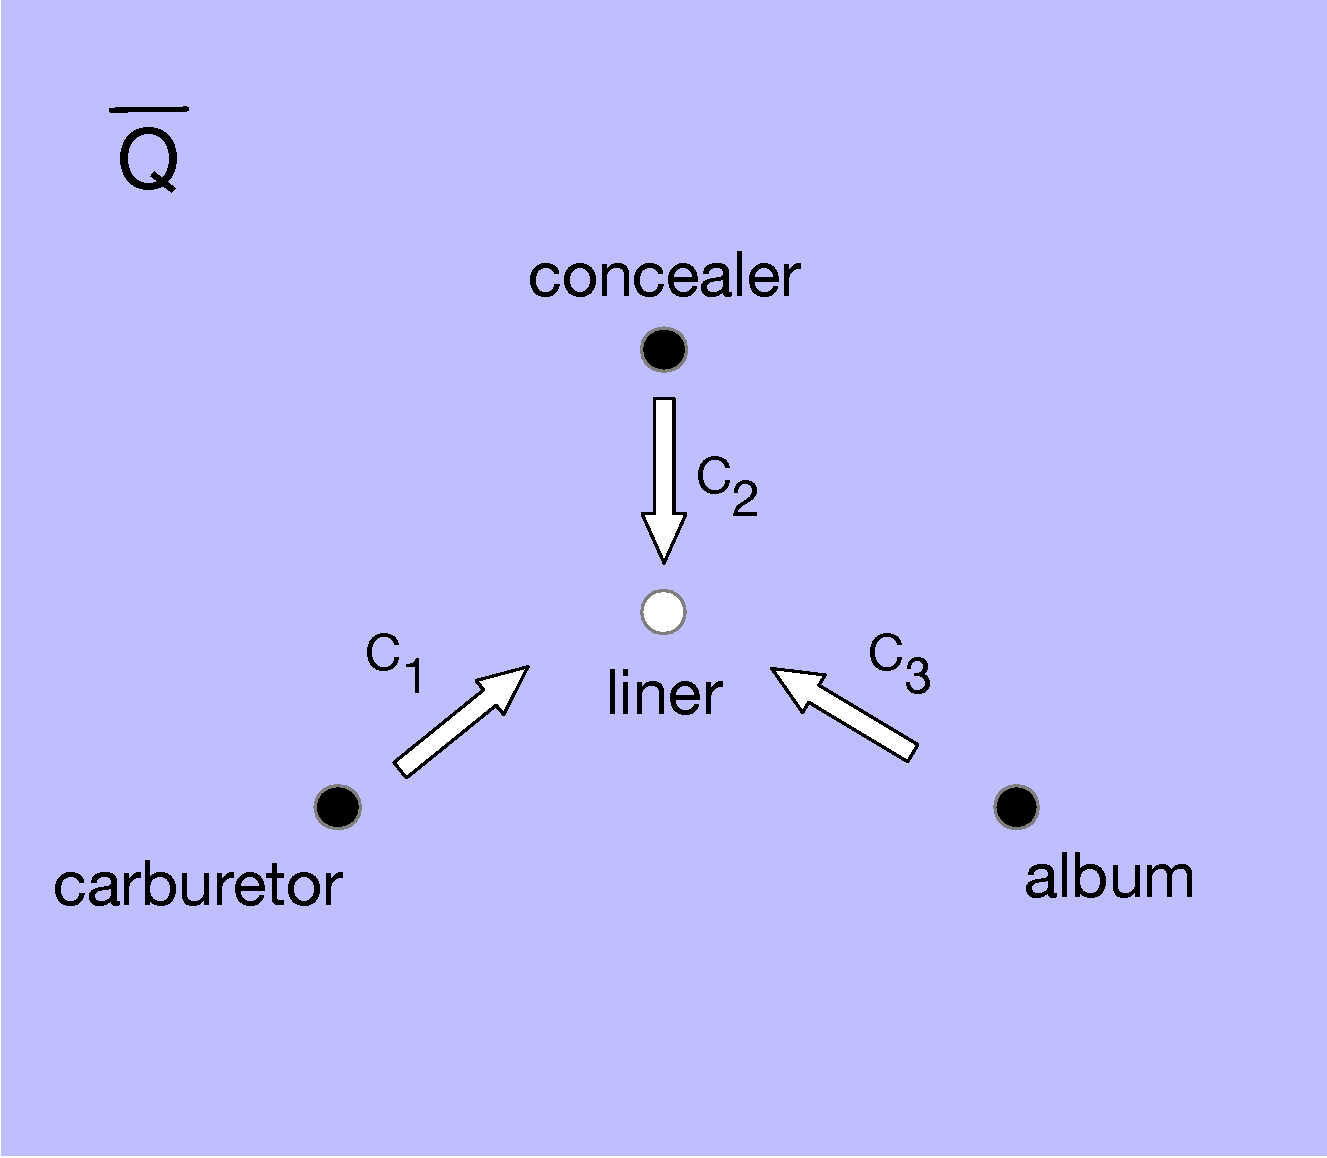
\includegraphics[width=0.5\textwidth]{combination.pdf} 
\onslide<2>
\begin{align*}
\bar{Q}_{\text{liner}} &\approx C_1 \bar{Q}_{\text{carburetor}} + C_2 \bar{Q}_{\text{concealer}} + C_3 \bar{Q}_{\text{album}} \\
&= 0.4 * \begin{bmatrix} 0.3 \\ \cdots \\ 0.1 \end{bmatrix} + 0.2 * \begin{bmatrix} 0.1 \\ \cdots \\ 0.2 \end{bmatrix} + 0.4 * \begin{bmatrix} 0.1 \\ \cdots \\ 0.4 \end{bmatrix} 
\end{align*}
\end{figure}
\end{frame}



\begin{frame}{Anchoring}
\begin{itemize}
\item If an anchor word appears in a document, then its corresponding topic is among the set of topics used to generate document~\citep{arora-2012-anchor}.
\item Anchoring algorithm uses word co-occurrence to find anchors and gradient-based inference to recover topic-word distribution~\citep{arora-2013}.
\item Runtime is \textbf{fast} because algorithm scales with number of unique word types, rather than number of documents or tokens.
\end{itemize}
\end{frame}

\begin{frame}{Anchoring}
\begin{enumerate}
\item<1-> Construct co-occurrence matrix from documents with vocabulary of size $V$: 
\[
\bar{Q}_{i,j} = p(w_2 = j \g w_1 = i).
\]
\item<2-> Given anchor words $s_1,...,s_K$, approximate co-occurrence distributions:
\[
\bar{Q}_i \approx \sum\limits_{k=1}^K C_{i,k} \bar{Q}_{s_k} \text{ subject to } \sum\limits_{k=1}^K C_{i,k}=1 \text{ and } C_{i,k} \ge 0.
\]
\item<3-> Find topic-word matrix:
\begin{align*}
A_{i,k} &= p(w=i \g z=k) \propto p(z=k \g w=i) p(w=i)\\
 &= C_{i,k} \sum\limits_{j=1}^V \bar{Q}_{i,j}.
\end{align*}
\end{enumerate}
\end{frame}

\begin{frame}{Finding Anchor Words}
\begin{itemize} 
\item So far, we assume that anchor words are given. 
\item How do we find anchor words from documents?
\end{itemize}
\end{frame}

\begin{frame}{Finding Anchor Words}
\begin{figure}
\begin{overprint}
\onslide<1>\centerline{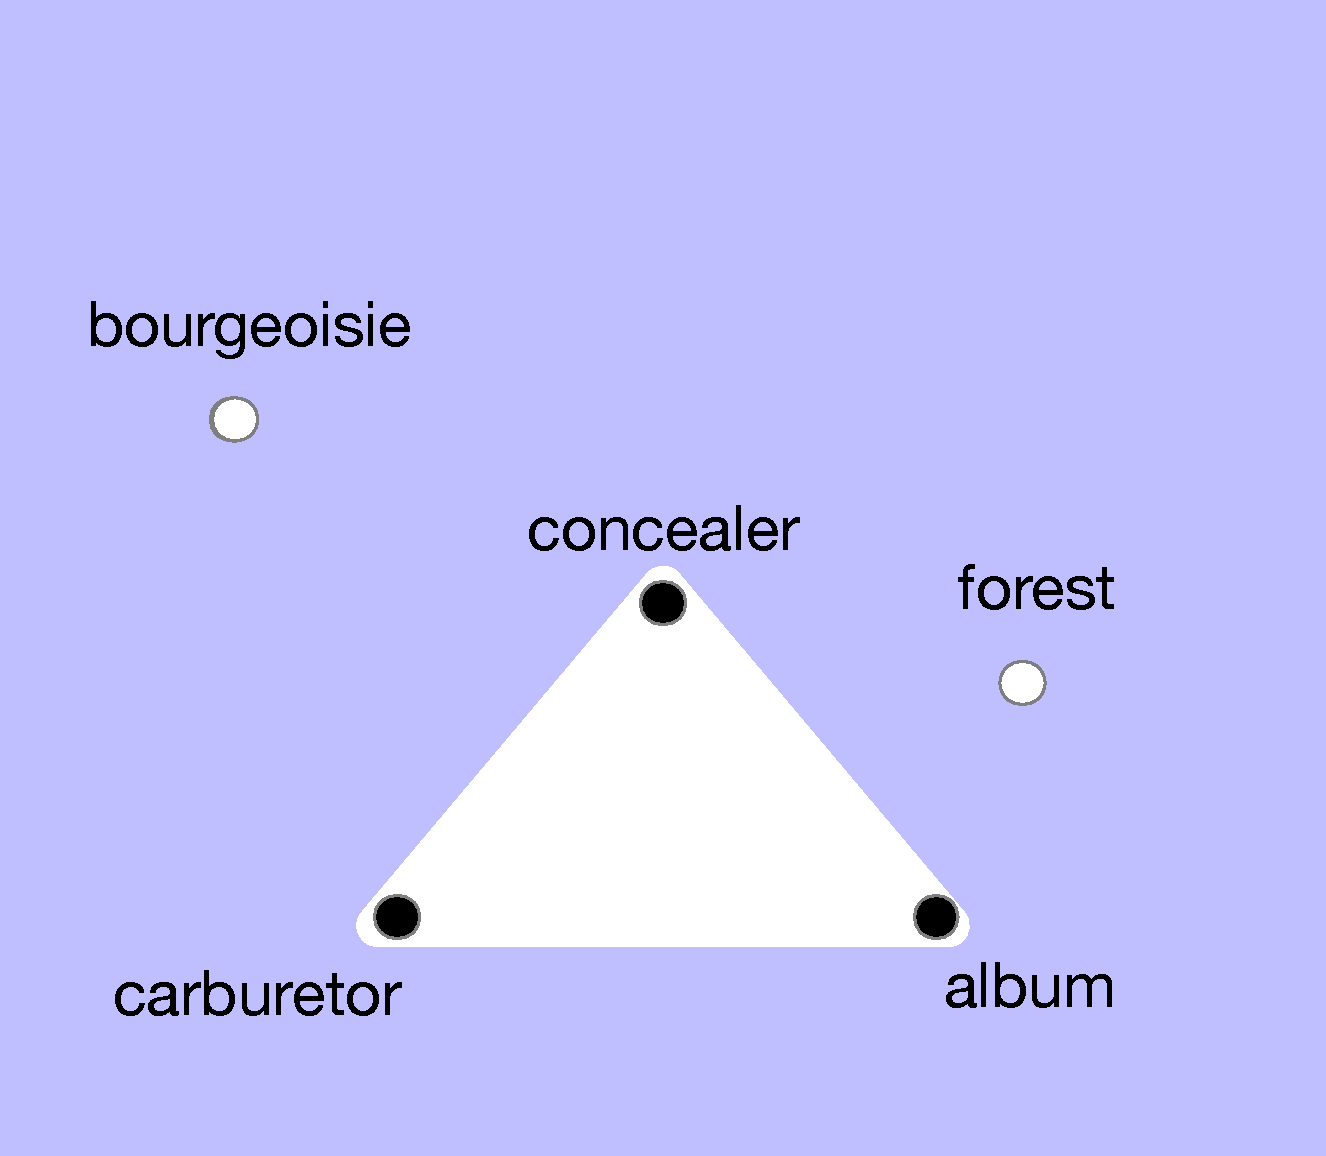
\includegraphics[width=0.7\textwidth]{mono_anchors1.pdf}}
\onslide<2>\centerline{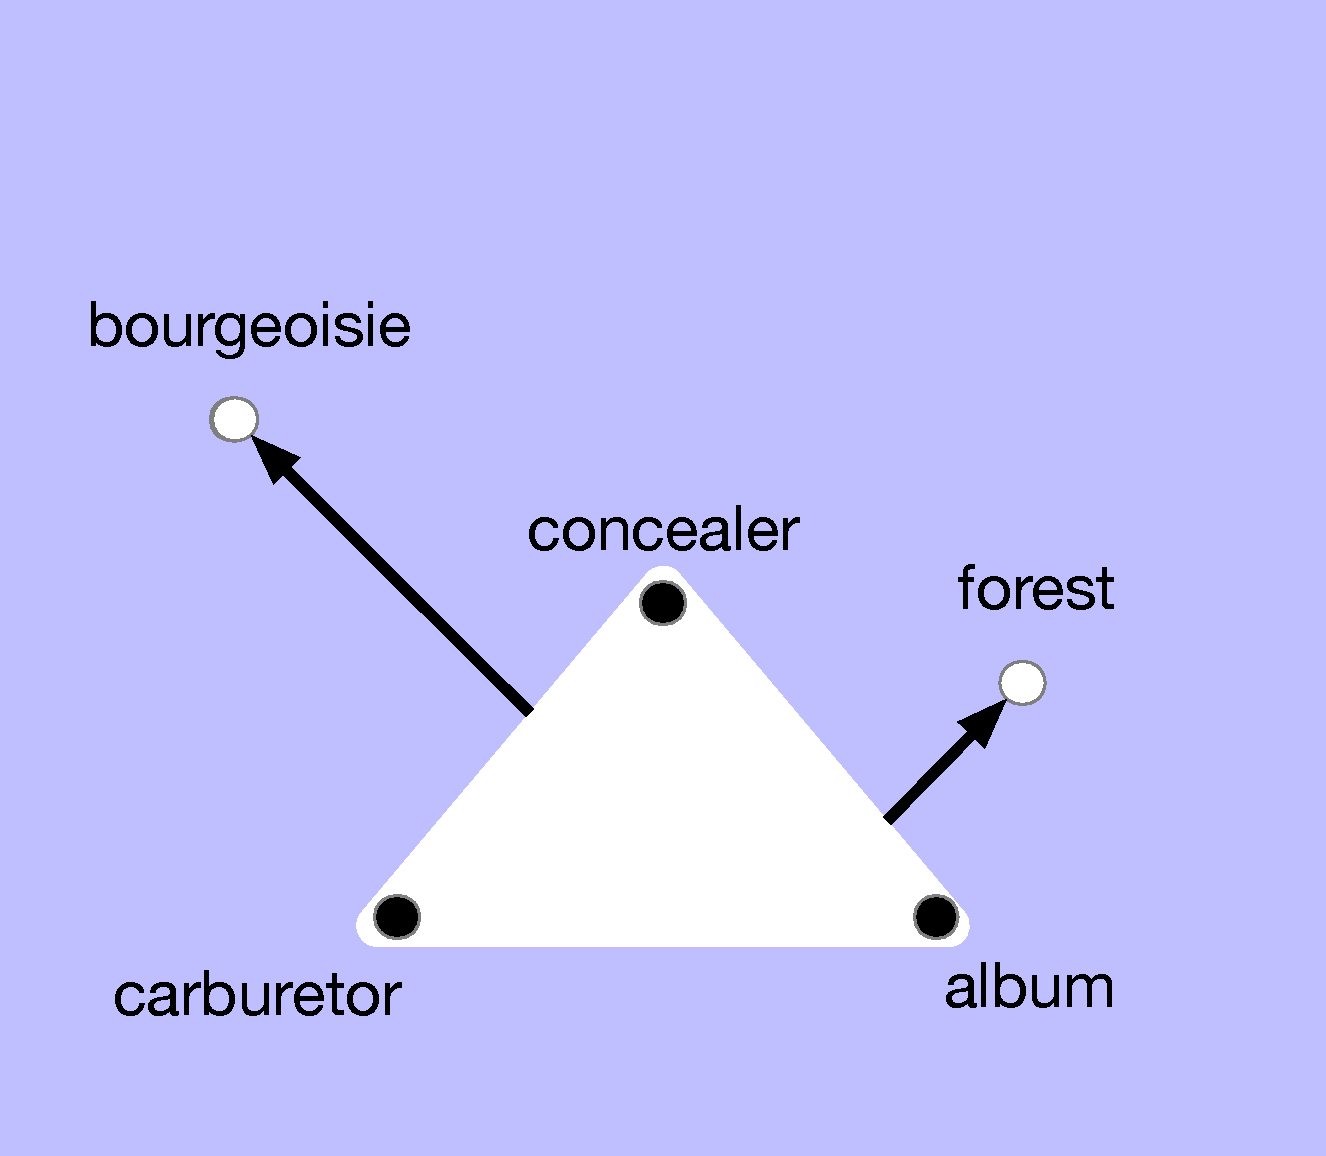
\includegraphics[width=0.7\textwidth]{mono_anchors2.pdf}}
\onslide<3>\centerline{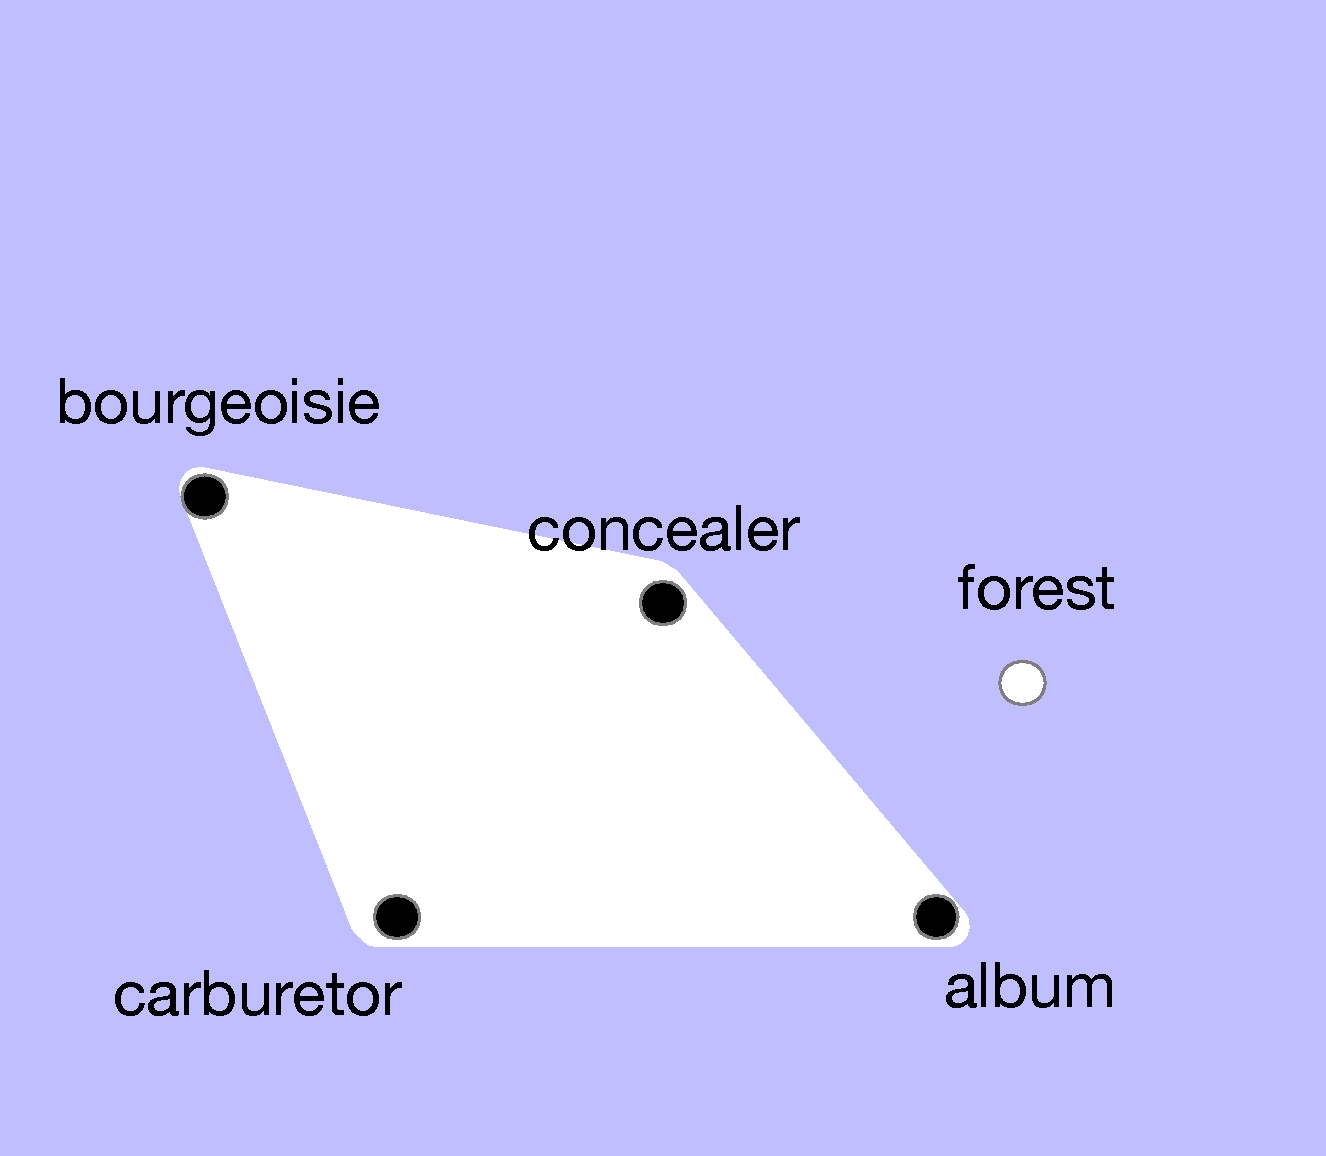
\includegraphics[width=0.7\textwidth]{mono_anchors3.pdf}}
\end{overprint}
\end{figure}
\center Anchor words are the vertices of the co-occurrence convex hull.
\end{frame}

\begin{frame}{Issues with Topic Models}
\begin{table}
\begin{tabular}{l} \\
Topics \\
\midrule
\textcolor<2>{color5}{music concert singer voice chorus songs album} \\
\textcolor<2>{color5}{singer pop songs music album chorale jazz} \\
cosmetics makeup eyeliner lipstick foundation primer eyeshadow \\
\end{tabular}
\end{table}
\onslide<2> 
\vspace{1cm} 
\begin{center}
\textbf{\textcolor{color5}{Duplicate topics.}} 
\end{center}
\end{frame}


\begin{frame}{Issues with Topic Models}
\begin{table}
\begin{tabular}{l} \\
Topics \\
\midrule
\textcolor<2>{color5}{music band art history literature books earth} \\
\textcolor<2>{color10}{bts taehyung idol kpop jin jungkook jimin} \\
\end{tabular}
\end{table}
\onslide<2> 
\vspace{1cm} 
\begin{center}
\textbf{\textcolor{color5}{Ambiguous topics.}} \\
\textbf{\textcolor{color10}{Overly-specific topics.}}    
\end{center}
\end{frame}

\begin{frame}{Interactive Anchoring}
\begin{itemize}
\item Incorporating interactivity in topic modeling has shown to improve quality of model~\citep{hu-2014-itm}.
\item Anchoring algorithm offers speed for interactive work, but single anchors are unintuitive to users. 
\item \textbf{Ankura} is an interactive topic modeling system that allows users to choose multiple anchors for each topic~\citep{lund-2017}. 
\item After receiving human feedback, \textbf{Ankura} only takes a few seconds to update topic model. 
\pause
\vspace{1cm}
\end{itemize}
\textbf{These methods only work for monolingual document collections.}
\end{frame}